\chapter{Fundamentals and Applications of Computer Architectures and Compiler Design}
\label{ch:methods}

\section{Hardware Implementation of Neural Networks}
This thesis mainly focuses on a processor that is an essential part of the \textbf{\ac{HICANN-DLS}} chip.
The following chapter will deal with the \ac{HICANN-DLS} as a whole and then look into the \textbf{\ac{PPU}} in detail while also addressing processor architecture in general.

The \ac{HICANN-DLS} was built to emulate neural networks at high speeds with low power consumption.
In contrast to many other systems \reference{other systems} it is a \textbf{spike based} system.
This means that neuronal activities do not follow discrete time steps and neurons send out spikes when activated.

Neurons are interconnected through dendrites, synapses and axons where synapses can be of different coupling strength. 
This means that a neuron is activated only for a short time, called a spike, and sends out this spike through its axon to neurons that are connected via synapses.
Between those spikes the neuron is resting and not sending any signals while still receiving input spikes from other neurons.
Synapses can work quite differently but have in common that there is a certain weight associated to them, which we will call synaptic weight.
The synaptic weight either amplifies or attenuates the pre-synaptic signal.
The signal is then passed through the dendrite of the post-synaptic neuron to the soma where all incoming signals are integrated.
If the integrated signals reach a certain threshold the neuron spikes and sends this signal to other neurons~\citep{silbernagl2009color}.

The \ac{HICANN-DLS} system implements a simplified neural model in analog electronics in order to emulate neuronal networks in a biologically plausible parameter range.

\begin{figure}[h!]
    \centering
    %
\noindent{\begin{minipage}{\textwidth}
   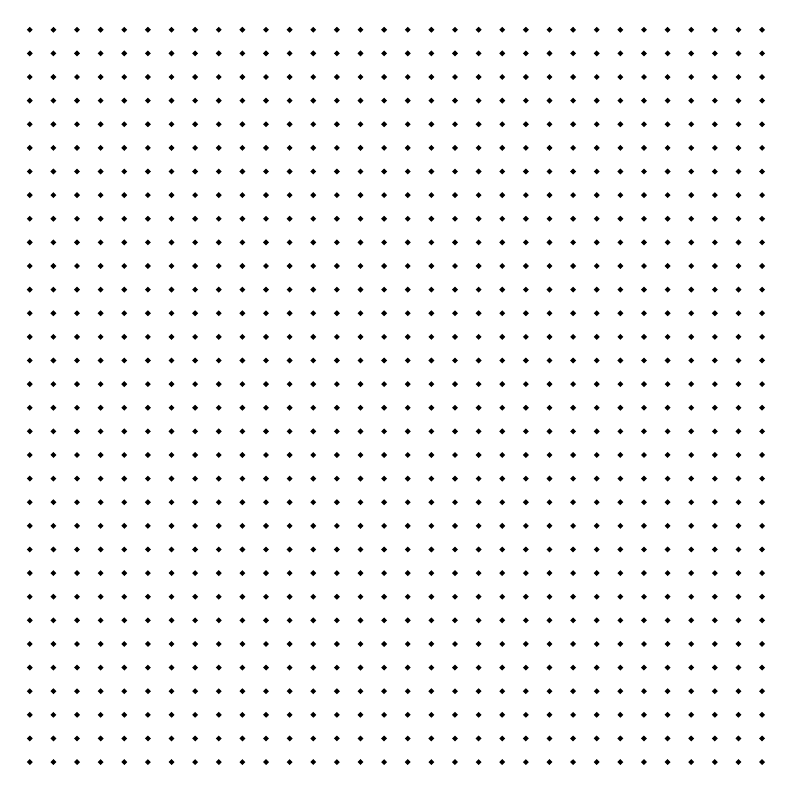
\begin{tikzpicture}[style={circle,draw,fill=black,minimum size=15}, line width=.5mm]
       \foreach \x in {0,...,31}
           \foreach \y in {0,...,31} 
                  {\pgfmathtruncatemacro{\label}{\x - 5 *  \y +21}
                  \node [circle,draw,fill=black,minimum size=0.1, inner sep = 0pt]  (\x\y) at (0.3*\x,0.3*\y) {};}
   \end{tikzpicture}
\end{minipage}}

    \caption{\label{fig:array} The synaptic array consists of pre-synaptic inputs (left), neurons (bottom) and 1024 synapses. All synapses along a column are connected to the respective neuron. Pre-synaptic inputs send their signal to all synapses along their respective row.}
\end{figure}
At its core it has a so called \textbf{synaptic array} (see figure~\ref{fig:array}) that connects 32 neurons which are located on a single chip to 32 different pre-synaptic inputs).
They enclose a 2D field which is the synaptic array as it mainly consists of synapse circuits.
All neurons reach into the array through input lines that are organized in columns.
The pre-synaptic inputs respectively have wires that resemble rows in the array.
At each intersection of those rows and columns, a synapse is placed that thereby connects a neuron and a pre-synaptic input.
Overall this gives 1024 synapses that interconnect neurons with the synaptic input.

A \textbf{\ac{FPGA}} is connected to all pre-synaptic inputs and routes external spikes to these inputs.
Synapses are realized as small repetitive circuits that contain 16 bits of data (see figure~\ref{fig:circuit}).
6 bits of those are used as \textbf{synaptic weight} and the spare two upper bits of that byte are used for calibration.
Each synapse also holds a 6-bit wide internal decoder address.
Decoder Address and synaptic weight can both be changed from outside.

The synapse array can also be used in 16-bit mode for higher weight accuracy, that combines the weights of two synapses to a 12-bit weight.
\begin{figure}[htbp]
    \centering
    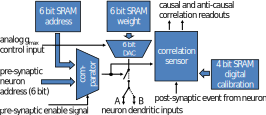
\includegraphics[width=\textwidth]{pictures/syncircuit.pdf}
    \caption{\label{fig:circuit} Block diagram of a synapse circuit (modified from \citeauthor{PPU}).}
\end{figure}

The \ac{FPGA} sends a 6-bit address whenever it sends a spike to a pre-synaptic input which then is compared by each synapse to the decoder addresses they hold themselves.
In case the addresses match, each synapse multiplies an output signal with the weight it stores and sends the result along a column where it reaches the neuron.
Along those columns signals from different synapses are collected.
Inside the neurons the resulting current input is integrated and if it exceeds a certain threshold the neuron spikes.
If the neuron is spiking it sends an output signal to the FPGA which is responsible for spike routing in the first place.
All of this is done continuously and does not follow discrete time steps, as mentioned earlier.
Along each column sits a \textbf{\ac{CADC}} that measures correlation of post- and pre-synaptic spikes and can be accessed by the \ac{PPU} similar to the synaptic array.
\begin{wrapfigure}[15]{l}{0.5\textwidth}
\captionsetup{format=plain, indention=.6cm, labelsep=newline,singlelinecheck=false}
    \centering
    \includegraphics[width=0.5\textwidth]{pictures/nux.pdf}
    \caption{\label{fig:nux} Block diagram of the nux architecture (modified from \citeauthor{PPU}).}
\end{wrapfigure}
The \ac{PPU} is the processing unit of \ac{HICANN-DLS} and is equipped with a \ac{VE} that is called \ac{s2pp}.
It is also connected to the digital information is the synapse array.

The following naming convention will be used throughout this thesis:
\begin{description}
    \item[\ac{PPU}] is the processor which is part of \ac{HICANN-DLS} and mainly responsible for plasticity.
    \item[nux] refers to the architecture of the \ac{PPU}, see figure~\ref{fig:nux}.
    \item[\ac{s2pp}] describes the \ac{PPU}'s \ac{VE} and is part of the nux architecture.
\end{description}

Digital configuration of the synapses and writing \ac{PPU} programs to the memory is handled by an \ac{FPGA}, that has access to every interface of a \ac{HICANN-DLS} chip.

It was developed to handle plasticity and can apply different plasticity rules to synapses during or in between experiments.
This is done much faster by the \ac{PPU} than by the \ac{FPGA} which is important for achieving experimental speeds that are $10^{3}$ times faster than their biological counterparts.
In general the \ac{PPU} is meant to handle plasticity of the synapses during experiments while the \ac{FPGA} should be used to initially set up an experiment, manage spike input and record data.


\section{Processor Architectures and the Plasticity Processing Unit}
Although the main goal of \ac{HICANN-DLS} is to provide an alternative analog architecture, there are advantages to classic computing which are needed for some applications and almost all contemporary processors are built using the so called von-Neumann architecture (figure~\ref{fig:processor}). \todo{add reference}

The main advantage of digital systems over analog systems, such as the human brain, is the ability to do numeric and logical operations at much higher speeds and precision as well as the availability of existing digital interfaces.
For this reason ``normal'' processors are responsible for handling experiment data as well as configuration of an experiment in the \ac{HICANN-DLS}.
We will now shortly get in touch with basics of such processors and explain common terms while referring to the \ac{PPU} at times when it is convenient.
\begin{wrapfigure}[20]{r}{0.5\textwidth}
\captionsetup{format=plain, indention=.6cm, labelsep=newline,singlelinecheck=false}
    \centering
        \vspace*{17mm}
        \chapter{Processor basics}
\label{chapter:processor}

Next to all processors used these days are built upon the so called von-Neumann architecture \todo{add reference}.
\todo{cite freidmann dissertation}Though the main goal of this group is to provide an alternative analogue architecture that is inspired by nature, there are advantages to the classic model of processors which are needed at some point.
The main advantage of digital systems over analogue systems such as the human brain, is the ability to do calculations at much higher speeds.
For this reason ``normal" processors are responsible for handling experiment data as well as setting up different parts of the experiment.
One such task is applying learning rules to the synapses during or in between experiments which can either be done by hand or with the help of the aforementioned PPU.
The second option is especially valuable when updating synaptic weights during an experiment as the PPU does this much faster than a system which interacts from the outside.
This is important for achieving experimental speeds that are $10^{4}$ times faster than their biological counterparts.

Therefore the PPU is one of many von-Neumann processors in this world and follows the same basic concepts.
It is important to understand these concepts as they build the foundation to this report!



ALU
FPU
memory
memory controller
clockcycle
pipeline


        \vspace*{-10mm}
        \caption{\label{fig:processor} Structure of a Processor in \\ von-Neumann Architecture}
\end{wrapfigure}
\\
The \ac{PPU}, which was designed by \citeauthor{PPU}, is a custom processor, that is based on the Power Instruction Set Architecture (PowerISA), which was developed by IBM since 1990. 
Specifically the \ac{PPU} uses POWER7 which was released in 2010 as a successor of the original POWER architecture.
It runs at 100 MHz clock frequency.

%general stuff
In general a microprocessor can be seen as a combination of two units which are an operational section and a control section.
The control section is responsible for fetching instructions and operands, interpreting them, controlling their execution and reading/writing to the main memory or other buses.
The operational section on the other hand creates results from instructions and operands as it performs logic or arithmetic operation on these, as instructed by the control section.
Prominent parts of the operational section are the \textbf{\ac{ALU}} and the \textbf{\ac{RF}}.

%register
The \ac{RF} can be seen as short-term memory of the processor.
It consists of several repeated elements, called \textbf{registers}, that save data and have share the same size which is determined by the architecture; the 32-bit architecture of nux for instance has 32-bit wide registers.

Typically the number and purpose of registers varies for different architectures.
Common purposes of registers are:
\begin{description}
    \item[\ac{GPR}] These registers can store values for various causes but in most cases are soon to be used by the ALU. Most registers on a processor are typically \ac{GPR}s.
        Any register that is not a \ac{GPR} is called a \textbf{\ac{SPR}}
    \item[\ac{LR}] This register marks the jump point of function calls. After a function completes, the program jumps to the address in the link register.
    \item[\ac{CR}] This register's value is set by an instruction that compares one or two values in GPRs. Its value can condition some instructions if they are executed or not.
\end{description}        
The \ac{ALU} uses values which are stored in the \ac{RF} to perform the aforementioned logic or arithmetic operations and saves the results there as well.

Some architectures also have an accumulator that is often part of the \ac{ALU}.
Intermediate results can be stored there because access to the accumulator is the fastest possible but it can only holds a single value at a time.
\\
\\

%memory
Memory of a von-Neumann machine contains both, the program and data.
Usually this memory is displayed as equal-sized blocks of information with addresses as in figure~\ref{fig:memory}.
\begin{figure}[htpb]
    \centering
    \begin{bytefield}[endianness=little]{32}
        \bitheader{0,7}\\
        \wordbox{1}{\tt 0x0001}\\
        \wordbox{1}{\tt 0x0002}\\
        \wordbox{1}{\tt 0x0003}\\
        \wordbox[]{1}{$\vdots$} \\[1ex]
        \wordbox{1}{\tt 0x3fff}\\
        \wordbox{1}{\tt 0x4000}\\
    \end{bytefield}
    \caption{\label{fig:memory} Illustration of Word Sizes for 32-bit Words}
\end{figure}

Because the smallest amount of information which we are interested in is usually a byte, each address is equivalent to one byte in memory.
The program is normally in a different location in memory than data and the processor goes through the program step by step. 
Each of these steps is called a machine instruction, which consists of several elements that occupy a fixed amount of memory (see figure~\ref{fig:opcode}).
\begin{figure}[htpb]
    \centering
    \begin{bytefield}[endianness=big, bitwidth=0.027777\linewidth]{32}
        \bitheader{0,7,15,23,31}\\
        \bitboxes{8}{{opcode}{operand 0 \\ \tiny{return operand}}{operand 1}{operand 2}}
    \end{bytefield}
    \caption{\label{fig:opcode} Representation of a Machine Instruction in Memory}
\end{figure}

%instructions
An instruction like in figure~\ref{fig:opcode} is called a \textbf{machine instruction} and combines several elements.
A program is simply a list of these instructions in memory that belong to the \textbf{instruction set}.
Each machine instruction requires a fixed amount of memory and consists of an opcode and multiple operands.
The \textbf{opcode} is the first part of the instruction and is typically an 8-bit number that identifies the operation.

Opcodes are often represented by an alias string like |add|, that is called a \textbf{mnemonic}.
The opcode is followed by several addresses that refer to the location a value can be taken from or where it should be stored.
These addresses are called \textbf{operands} and can either be a memory address or a register number.
The ALU reads this the opcode and operands and performs a set of so called \textbf{micro instructions} accordingly.

During a single clock cycle a chip can perform a single micro instruction.
An example for micro instructions in an add instruction (|d = add(a,b)|) would be:\citep[p.~23ff.]{microprocessor}
\begin{lstlisting}[caption=example of micro instructions, label=lst:microinstruction]
    1. fetch instruction from memory
    2. decode instruction
    3. fetch first operand a
    4. fetch second operand b
    5. perform operation on operands
    6. store result
\end{lstlisting}\todo{inhaltlicher zusammenhang}

%instruction set
The complexity of an instruction set is important for performance. 
As complex instruction sets feature highly specialized circuits and microinstructions, they are able to complete complex computation in only a few clock cycles.
But most often a complex instruction set would often rely a small set of basic arithmetic instructions and rarely use complex ones.
Because every micro instruction must be represented by a circuit in the \ac{ALU}, a smaller instruction set would safe space and be easier to design.
In general developing a processor architecture involves factors like: available chip space, instruction set and design complexity, energy consumption and maximum clock frequency.\unsure {give reason for clock frequency}
Because of this, processors can be classified in two main groups:
\begin{description}
    \item[\ac{CISC}] e.g. x86, MC68000, and i8080
    \item[\ac{RISC}] e.g. \ac{POWER}, ARM and MIPS
\end{description}
The latter usually has an instruction set that is reduced to simple  instructions like |add| or |sub| and connects these to create more complex instructions.
This is similar to how micro instructions work and makes programs on a \ac{RISC} processor more complicated, which also affects developers directly.
The architecture also features more registers than \ac{CISC} and instruction pipelining, which will be discussed later on.

The \ac{PPU} is a \ac{RISC} architecture so we will focus more on \ac{RISC}'s key features throughout this chapter.

%assembly
Programs that only consist of machine instructions a called \textbf{assembly} which is the lowest level of representation of a program that is still is human-readable.
Assembly instructions follow the same scheme as machine instructions do:
\begin{figure}[htpb]
    \centering
    \begin{bytefield}[endianness=big, bitwidth=0.027777\linewidth]{32}
        \bitheader{0,7,15,23,31}\\
        \bitboxes{8}{{mnemonic}{operand}{operand}{operand}}\\
        \bitheader{0,7,15,23,31}\\
        \bitboxes{8}{{\tt{addi}}{{\tt r1} \\ \tiny register address}{{\tt r2} \\ \tiny register address}{{\tt 5} \\ \tiny immediate operand}}
    \end{bytefield}
    \caption{\label{fig:mnemonic} Representation of Assembly Instruction {\tt addi} as a Machine Instruction in Memory. It adds an immediate value to register {\tt r2} and writes the result in {\tt r1}. Table~\ref{tab:asm} shows a list of important instructions in the PowerISA.}
\end{figure}

\begin{lstlisting}[caption=Assembly in Written Form, label=lst:asm]
addi     r1, r2, 5
\end{lstlisting}
In \ac{RISC} architectures instructions typically consist of 3 operands and are usually between registers only (except for load/store memory instructions).
Instructions that have less operands are usually mapped on different instructions.
Its operand can be of two different types which are all shown in figure~\ref{fig:mnemonic}.
They either represent a specific register (r1 = register 1) or an immediate value (5 = the integer 5).
\ac{RISC} architectures often also support only one \textbf{load} (memory to register) and one \textbf{store} (register to memory) instruction, which qualifies them as load/store architectures.
In order to access memory, operands must be used indirectly:

A memory address is given by an immediate value that is saved to a register.
A memory instruction then uses the value that is saved in the register instead of the register address as in listing \ref{lst:loadstore}.

\begin{lstlisting}[caption=Example Code for Load and Store Instruction. The contents of memory address {\tt 0x0000} are loaded into register {\tt r0} and then stored at address {\tt 0x1000}. See table~\ref{tab:asm} for information on used mnemonics., label=lst:loadstore]
li      r1, 0x0000
lw      r0, 0(r1)
li      r1, 0x1000
stw     r1, 0(r1)
\end{lstlisting}

It takes up to several hundred cycles for instructions to access memory which effectively stalls the processor until the memory instruction has finished.
\begin{equation*}
    \text{speed(accumulator)} > \text{speed(register)} \gg \text{speed(memory)}
\end{equation*}
Therefore a user should try to avoid memory access as much as possible and use registers instead.

As address size is limited by the register size, the maximum amount of memory that can be used is:\unsure{keep this?}
\begin{equation}
    2^{n} byte \xrightarrow{\text{n = 32 bit}} 2^{32} byte \approx 4*10^{9} byte = 4 GiB
\end{equation}

%pipiling
Since instructions on \ac{RISC} are all very simple, they also follow the scheme in listing~\ref{lst:microinstruction}.
The processor therefore start ``pipelining'' instructions, which means starting the next machine instruction as the previous machine instruction just performed the first micro instruction after one clock cycle.
Ideally, this will increase the performance by a factor that is equal to the number of micro instructions in a machine instruction.

It must be noted though, that the processor has to implement detection of \textbf{hazards}, which are data dependencies between instructions; e.g. one instruction needs the result of another.
Such an instruction is then postponed to a delay-slot and other instructions that do not cause hazards are executed instead.
The result is reordering of instructions on a processor level.
\\
\\
Processors sometimes have so called \textbf{co-processors} for complex instructions that are not included in the instruction set, but are still useful.
An example would be multiplication on most RISCs, which would need many cycles when split in |add| instructions.
A co-processor can perform this in just a few cycles.
In such a case the control section recognizes the |mult| opcode and passes it to the co-processor instead of the ALU.

This can be extended to whole units similar to the ALU existing in parallel.
One example would be a \textbf{\ac{FPU}} which is nowadays standard for most processors and handles all instructions on floating point numbers.
For this reason has the FPU its own \textbf{\acp{FPR}} in a separate register file.

A different kind of extension are vector extensions that do the same as the FPU but for vectors instead of floats and allows for \textbf{\ac{SIMD}} processing.
This is mostly wanted for highly parallel processes such as graphic rendering or audio and video processing \todo{reference}.
Early supercomputers such as the Cray-1 \todo{reference} also made use of vector processing to gain performance by operating on multiple values  simultaneously through a single register.
This could either be realized through a fully parallel architecture or more easily through pipelining instructions for vector elements.
The latter one is possible since there are typically no dependencies, hence no hazards, between single elements in the same vector.
Nowadays basically all common architectures support vector processing.
A few examples are:

\noindent\begin{minipage}[t]{\textwidth}
    \vspace{1em}
    \begin{minipage}[t]{0.4\textwidth}
\begin{itemize}
    \item x86 with SSE-series and AVX
    \item IA-32 with MMX
    \item AMD K6-2 with 3DNow!
\end{itemize}
\end{minipage}
\begin{minipage}[t]{0.6\textwidth}
\begin{itemize}
    \item PowerPC with AltiVec and SPE
    \item ARM with NEON
\end{itemize}
\end{minipage}
    \vspace{1em}
\end{minipage}

The \ac{s2pp} \textbf{\ac{VE}} on the nux architecture is the \ac{PPU}'s distinct feature that allows for \textbf{\ac{SIMD}} operations on synaptic weights.
The \ac{VE} is only weakly coupled to the \ac{GPP} of the \ac{PPU}.
Both parts can operate in parallel while interaction is highly limited.
To handle the vector unit the instruction set was extended by 53 new vector instructions that partly share their opcodes with existing AltiVec instructions.
This renders no problem since the nux does not recognize AltiVec opcodes and most likely is not going to in the future.
The {\ac{VRF} contains 32 new vector registers which are each 128-bit wide~\citep{AltiVec}.
    This allows for either use of vectors with 8 halfword (see figure~\ref{fig:bitlength}) sized elements or 16 byte sized elements which are 128 bits long as seen in figure~\ref{fig:vectorlength}.
\begin{figure}[htpb]
    \centering
    \begin{bytefield}[endianness=little]{32}
        \bitheader{0,1,7,15,31}\\
        \colorbitbox{lightgray}{1}{\tiny bit} && \bitbox{31}{}\\
        \colorbitbox{lightgray}{8}{byte} && \bitbox{24}{}\\
        \colorbitbox{lightgray}{16}{half-word} && \bitbox{16}{}\\
        \colorbitbox{lightgray}{32}{word}\\
    \end{bytefield}
    \caption{\label{fig:bitlength} Illustration of Word Sizes for 32-bit Words}
\end{figure}

But we take also a special interest in the AltiVec vector extension itself which was developed by Apple, IBM and Motorola in the mid 1990's and is also known as \ac{VMX} and Velocity Engine for the POWER architecture. 
The AltiVec extension provides a similar single-precision floating point and integer SIMD instruction set.
Its vector registers can either hold sixteen 8-bit |char| (V16QI), eight 16-bit |short| (V8HI), four 32-bit |int| (V4SI) or single precision |float| (V4SF), each signed and unsigned.
\begin{figure}[htpb]
    \centering
    \begin{bytefield}[endianness=little, bitwidth=\widthof{\tiny Integer~}/8]{128}
        \bitheader{0,7,15,31,63,127}\\
        \begin{rightwordgroup}{V16QI}\bitboxes{8}{{QI}{\tiny Quarter \\ Integer}{}{}{}{}{}{}{}{}{}{}{}{}{}{}}\end{rightwordgroup}\\
        \bitheader{0,7,15,31,63,127}\\
        \begin{rightwordgroup}{V8HI}\bitboxes{16}{{HI}{\tiny Half \\ Integer}{}{}{}{}{}{}}\end{rightwordgroup}\\
        \bitheader{0,7,15,31,63,127}\\
        \begin{rightwordgroup}{V4SI}\bitboxes{32}{{SI}{\tiny Single \\ Integer}{}{}}\end{rightwordgroup}\\
        \bitheader{0,7,15,31,63,127}\\
        \begin{rightwordgroup}{V4SF}\bitboxes{32}{{SF}{\tiny Single \\ Float}{}{}}\end{rightwordgroup}\\
    \end{bytefield}
    \caption{\label{fig:vectorlength} Vector structures are 128 bits wide and split into common word sizes.}
\end{figure}

It resembles most characteristics of the \ac{s2pp} vector extension, like a similar VRF, and is already implemented in the PowerPC back-end of \ac{GCC}, but both \ac{VE}s also feature differences.

The \ac{s2pp} \ac{VE} features a vector accumulator of 128 bits width and a \ac{VCR} which holds 3 bits for each half byte of the vector, making 96 bit in total.
The bits represent the result of a previous comparison instruction for vector elements.
If the first bit is set, the compared element was larger than |0|, if it was less than |0| the second bit is set and if the element is equal to |0|, the third bit is set.
For more information see the nux manual \citep[p.~23]{nuxmanual}.

Instructions on the \ac{s2pp} \ac{VE} can be specified to operate only on those elements of a vector, that meet the condition in the corresponding bits in the \ac{VCR}, while the AltiVec \ac{VE} utilizes the \ac{CR} of the PowerPC architecture.
This does not allow for selective operations on individual elements through the \ac{CR}, but allows for checking if all elements meet the condition in a single instruction.
If element-wise selection is needed, AltiVec offers this through vector masks.
    
The AltiVec \ac{VE} has two register that are not featured on \ac{s2pp}.
The \ac{VSCR} is responsible for detecting saturation in vector operations and decides which floating point mode is used.
The \ac{VRSAVE} assists applications and operation systems by indicating for each \ac{VR} if it is currently used by a process and thus must be restored in case of an interrupt.
Both of these registers are not available in the \ac{s2pp} \ac{VE} but would likely not be needed for simple arithmetic tasks which the \ac{PPU} is meant to perform.

We already stated that all instructions of \ac{VE}s must first pass the control unit, which detects vector instructions and then passes them to the \ac{VE}.
These instructions then go into an instruction cache for vector instructions. \unsure{add instruciton cache?}
On nux the instructions then shortly stay in a reservation station that is specific for each kind of operation and thus allows for little out-of-order operation for instructions in these reservation stations which is illustrated in figure~\ref{fig:s2pp}.
This allows for performing some arithmetic operations on a vector during the process of accessing a different vector in memory.
This results in a faster processing speed as pipelining for each instruction is also supported.
Though the limiting factor for this remains the \ac{VRF}'s single port for reading and writing.
An even more limiting factor is the shared memory interface of the \ac{s2pp} and \ac{GPP}.
\begin{figure}[htbp]
    \centering
    \includegraphics[width=\textwidth]{pictures/s2pp.pdf}
    \caption{\label{fig:s2pp} Detailed structure of the \ac{s2pp} vector extension (taken from \citeauthor{PPU}).}
\end{figure}

Normally processors themselves do not keep track of memory directly.
This is usually done by a \textbf{\ac{MMU}} or a \ac{MC}.
It handles memory access by the processor and can provide a set of virtual memory addresses which it translates into physical addresses.
Most modern \ac{MMU}s also incorporate a cache that stores memory instructions while another memory instruction is performed.
It detects dependencies within this cache, which can be resolved there.
Ultimately, this results in faster transfer of data because the \ac{MMU} can return results, it knows from the cache, without accessing the memory.

Not all \ac{MMU}s support this though, which might lead to certain problems when handling memory.
If instructions are reordered due to pipelining while dependencies on the same memory address are not detected correctly, an instruction may write to memory before a different one could load the previous value it needed from there.
Another reason could be delayed instructions, which were mentioned earlier.
For this reason memory barriers exist.

A \textbf{memory barrier} is an instruction that is equal to a guard, placed in code, that waits until all load and store instructions issued to the \ac{MMU} are finished.
It therefore splits the code into instructions issued before the memory barrier and issued after the memory barrier.
This prohibits any instruction from being executed on the wrong side of the barrier due to reordering and thereby generally prevents conflicting memory instructions.

This kind of memory barrier is called |sync| which is used in listing~\ref{lst:sync}.
This and other memory barriers are also described in table~\ref{tab:asm}.

\begin{lstlisting}[caption=The memory barrier ensures that the first store has been performed before the second store is issued., label=lst:sync]
stw     r7,data1(r9)    #store shared data (last)
sync                    #export barrier
stw     r4,lock(r3)     #release lock
\end{lstlisting}

Using |sync| can result in up to a few hundred cycles of waiting for memory access to finish and therefore this should only be done if necessary.

The \ac{PPU}'s memory is 16 kiB which is accompanied by 4 kiB of instruction cache.\todo{add description to instruction cache}
Together with the \ac{PPU} this is called the plasticity sub-system.
The \ac{MMU} of this system is very simple as it does not cache memory instructions and also has matching virtual and physical addresses, thus memory barriers can become necessary at times.
\\
\\
Another feature of the \ac{PPU} is the ability to read out spike counts and similar information through a bus which is accessible through the memory interface of the \ac{MMU}.
It uses the upper 16 bits of a memory address for routing
These are available because the memory is only 16 kiB large which is equivalent to 16-bit addresses.
A pointer to a virtual memory address allows to read for example spike counts during an experiment.
This is done the same way for the whole chip configuration such as analog neuron parameters.
\\
\\
The memory bus is also accessible by the \ac{FPGA}.
This is needed for writing programs into the memory as well as getting results during, or after experiments.
It also allows for communication between a ``master'' \ac{FPGA} and a ``slave'' \ac{PPU}.

A \textbf{bus} is the connection between parts of a processor and used for data transfer.
Bus speeds are very high as they transport data in parallel such as the contents of a register.
Thus most buses should be as wide as a register of the processor.
But as buses of such width need much space, some architectures use narrower buses with fewer bits than a register and instead use two instructions to transfer the contents of a full register.
The upper half of the width is called \textbf{high order bits} and the bottom half is called \textbf{low order bits} for big-endian architectures.
Systems of this sort are described as 32/16-bit architecture, which means that registers are 32 bit wide while buses are only 16 bit wide.
As the higher order bits of registers are not as often used as the lower order ones, it is often enough to move the lower 16 bits.
This results in less performance loss than one would initially expected.\unsure{keep this?}

One of the main feature of the \ac{PPU} though is access to the synaptic array which is offered through an extra bus, which can be seen in figure~\ref{fig:s2pp}.
\\
\\
When using vector instruction for nux, one must always keep in mind that the weights in the synaptic array only consist of the latter 6 or 12 bits which are in a vector register and are right aligned.
\begin{figure}[htpb]
    \centering
    \begin{subfigure}[b]{\textwidth}
        \centering
    \begin{bytefield}[bitwidth=0.11111111\textwidth]{8}
        \bitheader[endianness=big]{0-7}\\
        \bitbox{1}{\color{lightgray}\rule{\width}{\height}} & \bitbox{1}{\color{lightgray}\rule{\width}{\height}} & \bitbox{1}{$2^{-1}$} & \bitbox{1}{$2^{-2}$} & \bitbox{1}{$2^{-3}$} & \bitbox{1}{$2^{-4}$} & \bitbox{1}{$2^{-5}$} & \bitbox{1}{$2^{-6}$}\\
    \end{bytefield}
    \caption{\label{subfig:synapse} }
    \end{subfigure}
    \begin{subfigure}[b]{\textwidth}
        \centering
    \begin{bytefield}[bitwidth=0.11111111\textwidth]{8}
        \bitheader[endianness=big]{0-7}\\
        \bitbox{1}{$-1$} & \bitbox{1}{$2^{-1}$} & \bitbox{1}{$2^{-2}$} & \bitbox{1}{$2^{-3}$} & \bitbox{1}{$2^{-4}$} & \bitbox{1}{$2^{-5}$} & \bitbox{1}{$2^{-5}$} & \bitbox{1}{$2^{-7}$}\\
    \end{bytefield}
    \caption{\label{subfig:fracVE} }
    \end{subfigure}
    \caption{\label{fig:fractional} Comparison of \ref{subfig:synapse} Representation of Weights in Synapses and \ref{subfig:fracVE} Fractional Representation of Vector Components for Fixed-Point Saturational Arithmetic}
\end{figure}

Figure~\ref{fig:fractional} displays the representation of values in the synapses and in vectors.
The weight is the sum of the values where the bits are set to one.
In contrast to this, the sign-bit changes its meaning when used in the vector unit and becomes a factor instead of a summand.
This is the reason why a user must shift the vector's elements when reading/writing to the synapse array, as only then do special attributes of instructions work properly.

An example would be instructions that rely on \textbf{saturation} which predefines a minimum and maximum value.
In case, the result is out-of-range, the instruction will return either the minimum or the maximum (whichever is closer).
For this to work properly the bit representation must match the intended one, which is the above mentioned fractional representation, and the values must also be correctly aligned.

An overview of all vector opcodes is provided in the nux manual \cite[ch.~5]{nuxmanual}, which is recommended as accompanying literature besides this thesis.
In general these vector opcodes are divided into 6 groups of instructions:
\begin{description}
    \item[modulo halfword/byte instructions] apply a modulo operation after every instruction which causes wrap around in case of an overflow at the most significant bit position.
        Each instruction is provided as halfword (modulo $2^{16}$) and as byte instruction (modulo $2^{8}$).
    \item[saturation fractional halfword/byte instructions] allow for the results only to be in the range $[-1, 1-2^{-7}]$ for byte elements and $[-1, 1-2^{-15}]$ for half-word elements.
    \item[permute instructions] perform operations on vectors that handle elements of vectors as a series of bits.
    \item[load/store instructions] move vectors between vector registers and memory or the synapse array.
\end{description}


\section{Basic Compiler Structure}
\label{section:compiler}

\begin{wrapfigure}[18]{r}{0.35\textwidth}
\captionsetup{format=plain, indention=.6cm, labelsep=newline,singlelinecheck=false}
    \centering
        \chapter{Compiler Structure}
\label{chapter:compiler structure}

This part explains the structure of a compiler only on a very shallow level. Therefore the reader is encouraged to read further literature as the knowledge of a compilers structure helps a lot in understanding the way a buillt-in functions works and what problems might occur.

As already hinted by the abstract, a compiler consists of a front-end and a back-end, but also a third part that is the middle-end. These three parts sit on top of each other with the front-end on top and the back-end at the bottom and pass down the program as it is translated and optimized or compiled. But communication between the parts does not go only one way and changes that are made in the back-end affect the front-end as well!
The first part of the compilation process is the translation of code which is written in some programming language into a so called Immediate Representation (IR) that looks the same for every front-end language and usually is never seen by the user. Any supported programming language (C, C++, Java…) is implemented in its own front-end that defines how the language is translated into IR. After that the IR is send to the middle-end, which generally optimizes the IR and then passes the code to the back-end. The back-end first executes further optimizations that are target-specific followed by allocatiing registers and handling relative memory. Finally the code is translated into the assembly language that is supported by the target.
After the code is compiled and emmited as an object file it is also linked, which means combining different objectfiles and and assigning absolute memory addresses to tehm. At last the binary file emmited by the linker is loaded into the memory of the processor and then can be executed.

Most Compilers that are used nowadays are built of three basic components which handle different steps in the process of converting human-readable programming language to machine-readable machine code. As does the GNU Compiler collection (GCC) which also can be seen as made of three main parts. The so called front-end, middle-end and back-end.
All three parts work more or less independently from each other and communicate over a compiler-specific „language“, which is described a the Intermediate Representation (IR). It is typically never seen by the user and exists for a fact in many different forms [reference] one of which is Register Transfer Language (RTL), which is the lowest-level IR used by GCC. It is the most interesting IR when working on a back-end and will get more attention later in this report. But in before that we need to understand the structure an functioning of a compiler in general.

The first mentioned Front-end resembles the main interaction point between the human programmer and the machine. Front-ends are usually divided by their respective programming languages such as C, C++, Java…  and have the main task of converting any programming language into unified IR, that can be passed to the middle-end in GIMPLE or GENERIC language. Therefore no matter which language you prefer, in an ideal case code, that is syntactically identical, should not differ after it is processed by the front-end. This is due to the goal of compilers such as GCC and LLVM to support as many languages and machines as reasonably possible while offering the equally good optimization and saving themselves overall work. It obvious that a single compiler for every combination of language and machine would simply not be practical, especially as the optimization taking place in the middle-end follows the same rules for pretty much any architecture.
The middle-end main task is basically this sort of optimization, and makes for the main difference between compilers as most compilers offer the same range of front-ends and back-ends. (Part about the optimizations taking place in the middle-end). After all optimizations are through, the middle-end passes IR in form of RTL to the back-end. As you can see the middle-end rarely needs to be modified except for fundamental changes in the compilers architecture such as new kinds of optimizations and „multiple memory handling“ (also Harvard-Architecture (vielleicht))
The back-end is responsible for the final steps of the compilation process as it translates the general RTL IR into specific Assembly commands. It uses some sort of table of available assembly instructions, that is provided, and finds the best fitting instructions. GCC for example uses a Lisp-like language (is this RTL?) that uses something called insns. These combine different properties with the  Assembly commands like an equivalent set of actions that are executed, the  operands and the constraints it must satisfy. These will be further explained later. The back-end also contains the the code which implements processor-specific built-in functions.
Depending on the Compiler architecture the back-end it finally emits IR to the assembler which emits the machine code in assembly or emits assembly itself. Then finally the linker links the assembly code of all program files together and substitutes the offset addresses with absolut addresses to generate the final machine code.
reload
register spilling
register handling
endianess
wordsize

different parts of an instruction, mention: opcodes, asm instruction, operation, operand, insn, IR, builtin function/intrinsic

        \caption{\label{fig:compiler} Compiler Representation}
\end{wrapfigure}
At its core every compiler translates a source-language into a target-language as figure~\ref{fig:compiler} illustrates.
Most often it translates a high-level, human readable programming language into a machine language that consists of basic instructions that build complicated structures.
In doing so, compilers may be the essential part in everyday lives of programmers everywhere.
Thereby compilers played a key role in development of computers in general.

What differs compilers from interpreters is the separation of \textbf{compile-time} and \textbf{run-time}.
As interpreters combine these two and translate a program at run-time, a compiler reads the source-language file completely (often several times) and only then creates the executable files which are executed after the process has finished.
The advantages of this are simple:
While a compiler takes some time at first until the program can be started, the resulting executable is next to always faster and more efficient.
This is due to the possibility of optimizing code during the compilation process and the chance of reading through the source file several times if this is needed (with each time the code is read being called a \textbf{pass}).
Of course there do exist many different compilers today and what matters to the user is typically the combination of the amount of time it takes to compile a program and the performance of that program.
\begin{figure}[htb]
    \centering
    \begin{subfigure}[t]{0.25\textwidth}
            \tcbset
    {my box/.style={enhanced,colframe=blue!70!black,colback=white!50!blue,colupper=red!50!black,
        fonttitle=\bfseries,nobeforeafter,center title, noparskip, size=small},
    every box on layer 1/.style={every box},
    every box on layer 2/.style={reset,my box}}
\begin{tcolorbox}[enhanced jigsaw, width=\textwidth, opacityframe=0.0, opacityback=0.0]
\begin{tcolorbox}[enhanced, height=.5cm, width=\linewidth, remember as=pp, opacityframe=0.0, opacityback=0.0]\end{tcolorbox}
\begin{tcolorbox}[enhanced, height=.7cm, width=\linewidth, watermark text=Preprocessor, remember as=pp]\end{tcolorbox}
\begin{tcolorbox}[tcbox raise base, width=\linewidth, enhanced jigsaw, remember as=cmp]
    \begin{tcolorbox}[enhanced, breakable, noparskip,opacityframe=0.3, opacityback=0.3, height=1.4cm, width=\linewidth, watermark text=Front-End, remember as=fe]
    \end{tcolorbox}
    \begin{tcolorbox}[enhanced, breakable, noparskip,opacityframe=0.3, opacityback=0.3, height=0.7cm, width=\linewidth, watermark text=Middle-End, remember as=me]
    \end{tcolorbox}
    \begin{tcolorbox}[enhanced, breakable, noparskip,opacityframe=0.3, opacityback=0.3, height=1.1cm, width=\linewidth, watermark text=Back-End, remember as=be]
    \end{tcolorbox}
\end{tcolorbox}

\end{tcolorbox}

\begin{tikzpicture}[overlay,remember picture,line width=1mm]
    \draw[->, shorten >=-1.5mm] ($(pp.north)+(0,1.5)$) -- node [left] {program code} (pp.north);
    \draw[->, shorten >=-1.5mm] (pp.south) -- (fe.north);
    \draw[->, shorten >=-1.5mm] (fe.south) -- (me.north);
    \draw[->, shorten >=-1.5mm] (me.south) -- (be.north);
    \draw[->] (be.south) -- node [left] {machine files} ++(0,-1.5);
\end{tikzpicture}

        \caption{\label{fig:cmpstruct} }
    \end{subfigure} \hspace{2cm}
    \begin{subfigure}[t]{0.37\textwidth}
        
    \tcbset
    {enhanced,colframe=blue!70!black,colback=white!50!blue,colupper=red!50!black,
    fonttitle=\bfseries,nobeforeafter,center title, noparskip}
            \begin{tcolorbox}[tcbox raise base, width=\linewidth, enhanced jigsaw, remember as=cp]
                \begin{tcolorbox}[enhanced jigsaw, breakable, noparskip,opacityframe=0.3, opacityback=0.3, width=\linewidth]
                    \begin{tcolorbox}[enhanced,center title,width=\linewidth, remember as=sc]
                        \begin{center}Scanner\end{center}
                    \end{tcolorbox}
                    \begin{tcolorbox}[enhanced,width=\linewidth, remember as=ps]
                        \begin{center}Parser\end{center}  
                    \end{tcolorbox}
                    \begin{tcolorbox}[enhanced, width=\linewidth, remember as=sa]
                        \begin{center}Semantic \\ Analyzer \end{center} 
                    \end{tcolorbox}
                    \begin{tcolorbox}[enhanced, width=\linewidth, remember as=sco]
                        \begin{center}Source Code \\ optimizer \end{center}
                    \end{tcolorbox}
                \end{tcolorbox}
                \begin{tcolorbox}[enhanced jigsaw, breakable, noparskip,opacityframe=0.3, opacityback=0.3, height=1cm, width=\linewidth, remember as=me, watermark text=Middle-End]
                \end{tcolorbox}
                \begin{tcolorbox}[enhanced jigsaw, breakable, noparskip,opacityframe=0.3, opacityback=0.3, width=\linewidth]
                    \begin{tcolorbox}[enhanced, width=\linewidth, remember as=cg]
                        \begin{center}Code Generator  \end{center}
                    \end{tcolorbox}
                    \begin{tcolorbox}[enhanced, width=\linewidth, remember as=tco]
                        \begin{center}Target Code \\ Optimizer \end{center}
                    \end{tcolorbox}
                \end{tcolorbox}
            \end{tcolorbox}
            \begin{tikzpicture}[overlay,remember picture,line width=1mm]
                \draw[->, shorten >=-1.5mm] ($(cp.north)+(0,1)$) -- (sc.north);
                \draw[->, shorten >=-1.5mm] (sc.south) -- (ps.north);
                \draw[->, shorten >=-1.5mm] (ps.south) -- (sa.north);
                \draw[->, shorten >=-1.5mm] (sa.south) -- (sco.north);
                \draw[-] (sco.south) -- (me.north);
                \draw[->, shorten >=-1.5mm] (me.south) -- (cg.north);
                \draw[->, shorten >=-1.5mm] (cg.south) -- (tco.north);
                \draw[->] (tco.south) -- ($(cp.south)+(0,-1)$);
            \end{tikzpicture}
            \begin{tikzpicture}[overlay,remember picture,line width=1mm]
                \draw[-, draw=blue!30!white,line width=.5mm, shorten >=.2cm,shorten <=.1cm] (cmp.north east) -- (cp.north west);
                \draw[-, draw=blue!30!white,line width=.5mm, shorten >=.2cm,shorten <=.1cm] (cmp.south east) -- (cp.south west);
            \end{tikzpicture}

        \caption{\label{fig:cmpintstruct} }
    \end{subfigure}
    \caption{\label{fig:cmp} Overviews of Compilation Stages \\ The compilation tree in \ref{fig:cmpstruct} has different contributors besides the compiler. The compiler in \ref{fig:cmpintstruct} goes through different phases, that belong to the front- or back-end.}
\end{figure}

A compiler is not the only contributor to translation of a program into an executable program although it is the most prominent one.
Figure~\ref{fig:cmpstruct} illustrates the chain of tools that is involved into this process:
First the \textbf{preprocessor} modifies the source before it is processed by the compiler and removes comments, substitutes macros and also includes other files into the source before it passes the new program code to the compiler.
The compiler then passes its output to the \textbf{assembler} which translates the output of the compiler which is written in a language called \textbf{assembly} into actual machine code by substituting the easy-to-read string alternatives with actual opcodes.
At last the \textbf{linker} combines the resulting ``object-files'' that the assembler emitted with standard library functions, that are already compiled, and other resources. 
The result is a single file that is almost executable.
The only task which is left for the \textbf{loader} is assigning a base address to the relative memory references of the ``relocatable'' file.
The code is now fully written in machine language and ready for operation.
\\
\\
Figure~\ref{fig:cmpintstruct} shows the separation of a compiler into \textbf{front-end}, \textbf{back-end} and an optional \textbf{middle-end}.
This is done to make a compiler portable, which means allowing the compiler to work for different source-languages which are implemented in the front-end and target-languages which must be specified in the back-end.
Therefore if one wants to compile two different programs e.g. one in C the other in FORTRAN, it is necessary to change the front-end but not the back-end because the machine or \textbf{target} stays the same.
The middle-end in this regard is not always needed but could be responsible for optimizations that are both source-independent and target-independent.

Of course the different parts of the compiler have to communicate through a language that all parts can understand or speak.
Such a language is called \textbf{\ac{IR}} and also used during different phases of the compilation process.
It may differ in its form but always stays a representation of the original program code.
\\
\\
The different phases of a compilation process are illustrated to the far right of figure~\ref{fig:compiler}.
First the preprocessed source code is given to the \textbf{scanner} that performs lexical analysis, which is combining sequences of characters and attributes such as ``number'' or ``plus-sign'' to so called tokens.
Next the \textbf{parser} takes the sequence of tokens and builds a syntax tree that represents the structure of a program and is extended by the \textbf{semantic analyzer} which adds known attributes at compile-time like ``integer'' or ``array of integers'' and checks if the resulting combinations of attributes are valid.
This already is the first form of \ac{IR}.
The \textbf{source code optimizer} which is the last phase of the front-end takes the syntax tree and takes a first shot at optimizing the code.
Typically only light optimization is possible at this point such as pre-computing simple arithmetic instructions.
After the source code optimizer is done the syntax tree is converted into different IR in order to be passed to the back-end.

The \textbf{code generator} takes this \ac{IR} and translates it to machine code that fits the target --- typically this is assembly.
At last the \textbf{target code optimizer} tries to apply target-specific optimization until the target code can be emitted.

During these phases the compiler also generates a symbol and literal table.
A \textbf{symbol table} is, as the name states, an overview of all symbols that are used in the program, it contains the symbols name and the attribute of the semantic analyzer.
A \textbf{literal table} in contrast holds constants (i.e. strings) and makes them globally available by reference, as does the symbol table.
This information is used by the code generator and various optimization processes.

\subsection{Back-End and Code Generation}
The last two phases of the compiler, which are part of the back-end, are the most interesting in respect to this thesis.
Usually the processes of code generation and target optimization in the back-end are entangled as optimization can take place at different phases of code generation.
Thus we first take a look at code generation in the back-end.
\\
\\
As we learned already, the source program reaches the back-end in form of \ac{IR}.
Often the \ac{IR} is already linearized and thereby again in a form that can be seen as sequence of instructions.
Because of this the \ac{IR} may also be referred to as Intermediate Code.
The process of generating actual machine code from this is again split into different phases:
\begin{itemize}
    \item instruction selection
    \item instruction scheduling
    \item register allocation
\end{itemize}

At first the back-end recognizes sets of instructions in intermediate code that can be expressed as an equivalent machine instruction.
Depending on the complexity of the instruction set a single machine instruction can combine several \ac{IR} instructions.
This may involve additional information that the front-end aggregated and added to the \ac{IR} as attributes.
Single machine instruction can combine several of these \ac{IR} instructions.
At the end of this, a compiler typically emits a sequence of assembly instructions which we will explain later on.
In order to fulfill this task the compiler needs the specifications of the target it compiles for.
This is called a target description and can contain things like specifications of the register-set, restrictions and alignment in memory and availability of extensions and functionalities.
The compiler also needs knowledge of the instruction set of a target, which is determined by the \ac{ISA} and is a list of instructions which are available and also their functionality.
The compiler picks instructions according to their functionality from this list and substitutes the \ac{IR} with this.
Ideally a back-end thus could support different back-ends just by exchanging the machine description and the \ac{ISA} as the basic methods of generating code are the same for most targets.

After the IR is converted into machine instructions the back-end now rearranges the sequence of instruction.
This needs to be done as different instructions take different amounts of time to be executed.
If a subsequent instruction depends on the result of a previous instruction the compiler now has two alternative approaches to solve this.
First it can simply stall the programs execution as long as the instruction is executed and feed the next instruction into the processor only when the dependency is solved.
This means that the compiler adds |nop|s before every instruction that needs to wait for an operand as |nop| tells the processor to wait until the previous instruction has finished.
For critical memory usage the compiler can also insert |sync|s as memory barriers before hazardous memory instructions.
Alternatively it can stall only the instruction which depends on the result which is currently computed but perform instructions that do not depend on the result in the mean time.
By doing so the scheduler increases performance noticeably and thus can be seen as part of the optimization process.
On \ac{RISC} architectures this is especially important as load and store instructions can take a few hundred clock cycles more than normal register instructions and pipelining depends mainly on the instruction sequence.
Thus the scheduler is also involved parallelization of code.
As a result of this a compiler would usually accumulate all load instructions at he beginning of a procedure and start computing on registers that already have a value while the others are still loaded.
This is done vice versa at the end of a procedure for storing the results in memory.
This process of course needs the compiler to know the amount of time it takes for an instruction to be executed and works hand in hand with hazard detection on processor level.

At last he compiler handles register allocation which also includes memory handling.
Typically the previous processes expect an ideal target machine which provides and endless amount of registers.
As in reality the processor only has $k$ registers the register allocator reduces the number of ``virtual registers'' or ``pseudoregisters'' that are requested to the available number of ``hard registers'' $k$.
For this to be possible the compiler decides whether a value can live throughout a procedure in a register or must be placed into memory because there are not enough registers available.
This results in the allocator adding load and store instructions to the machine code in order to temporarily save those registers in memory which is called ``spilling''.
It is obvious that this can hurt performance and therefore the compiler tries to keep spilling of registers to a minimum and also insert spill code at places where it delays other instructions as little as possible.
At he end of register allocation the compiler assigns hard registers to the virtual registers which are now only $k$ at a time.

During and after code generation the compiler also applies optimizations to the machine code.
Any optimization to the code though must take three things into consideration, which are safety, profitability and risk/effort.
The first thing which always must be fulfilled, is safety.
Only if the compiler can guarantee that an optimization does not change the result of the transformed code compared to the original code it may use this optimization!
Only if this applies the compiler may check for the profit of an optimization which most often is a gain in performance but could also be the size of the program.
At last the effort or time it takes for the compiler to perform this optimization and the risk of generating actually bad or inefficient code should be taken into account as well.
If optimization passes these three aspects it may be applied to the code.
In the end there exist some simple optimizations that always pass this test like the deletion of unnecessary actions or unreachable code, e.g. functions that are never called.
Another example would be the reordering of code like the scheduler did before or the elimination of redundant code, which applies if the same value is computed at different points and thus the first result simply can be saved in a register.
If a compiler knows the specific costs of instructions, it can also try to substitute general instruction with more specialized but faster instructions, like substituting a multiplication with 2 by shifting a value one position to the left.
There exist many more ways of optimization but we only want to explain one more kind of optimization which is called peephole optimization.

In \textbf{peephole optimization} the compiler only looks at small amounts of code at a time through a ``peephole'' and tries to find a substitution for the specific sequence of instructions it ``sees''.
If the sequence can be substituted the peephole optimizer does so, otherwise the peephole is moved one step and the new sequence is evaluated.
These substitutions must be specified by hand and are highly target-dependent in contrast to the optimizations which were mentioned before that are target-independent.

\subsection{Inline Assembly}
\label{section:asm}
Following a short introduction in the previous section, we want to spend a little time on assembly as it is useful to know how to program in assembly while using C.
This is called \textbf{inline assembly} and uses the function |asm|.
\begin{lstlisting}[caption= Exemplatory Assembly invkation, label=lst:inlineasm, float, floatplacement=htbp]
int dst, src1, src2;
asm volatile (  "add %0, %1, %2"
                : "=r" (dst)
                : "r" (src1), "r" (src2):);
return dst; /*would return src1 + src2*/
\end{lstlisting}

Listing~\ref{lst:inlineasm} would generate the instruction |add| in the assembly output of the compiler which would be followed by three operands.

First one must write an assembler template that is based on assembly.
The integer in |%n| indicates the order, in which the operands are specified after the assembler template.

Output operands are specified after the first |:| as a list of comma separated constraints and variables.
|"=r"| is such a constraint, that determines that the operand is to be stored in a register (|r| for register operand) and that the register is to be written (|=| this is called a modifier).
The variable in parentheses must be declared in before and must be of matching type (|float| would not be allowed in this case).

The second |:| separates the input operands, which are specified the same way.
|r| again stands for a register operand and the variable is in parentheses, the different operands are separated by commas.
The third |:| separates operands from clobbered (=temporarily used) registers which would also be in quotes, but these are optional arguments and not needed in this case.
|volatile| means that the compiler must not delete the following instructions due to optimization.

|asm (:::memory);| is a special operand and would indicate a memory barrier to the compiler, ergo the machine instructions previous to this line and the one following may not be interchanged.\unsure{keep this?}

\subsection{Intrinsics}
Intrinsics are sometimes also called built-in functions and resemble an intermediate form of inline assembly and a high-level programming language.
This means that by calling an intrinsic function, we tell the compiler to use a certain machine instruction that typically shares its name with the intrinsic.
What differs an intrinsic from |asm()| is that we do not need to specify constraints or registers classes but only need to keep an eye on the type of arguments.
One could easily mistake them for normal library functions but they are directly integrated into the back-end of a compiler and thus independent of the programming language.
In order to implement intrinsics into a back-end, the compiler needs certain knowledge of what the |asm| instruction does and what kind of operands it needs.

A typical field of application for intrinsics would be vectorization and parallelization of code through processor extensions.
Sometimes this is the sole option of using the machine instructions associated with them.

\subsection{GNU Compiler Collection}
\label{sec:GCC}
The \ac{GCC} is a compiler suite that supports different programming languages and targets.
Though normally it is seen as a build of \ac{GCC} supports a variety of front-ends while it was built for a specific target.
This target in most cases is the processor architecture on which the user runs the compiler.
But \ac{GCC} also supports the idea of a cross-compiler, which is the concept of compiling code on one machine but running the code on another machine that may be based on a different architecture.
One build of \ac{GCC} does not support different back-ends though and therefore \ac{GCC} must be built individually for every back-end, it wants to compile code for.
This is realized through a modular structure which follows the idea of a front-end, middle-end and back-end as was described in section \ref{section:compiler} although some information that belongs to a back-end is also needed at the front-end, hence the compiler is built back-end specific but supports a wide variety of back-ends to choose from.

\ac{GCC} itself is programmed in C++ and part of the GNU project of the Free Software Foundation.
It is wide-spread and one of the most popular compilers especially among academic institutions and small scale developers.
Every major UNIX distribution and many minor ones include \ac{GCC} as a standard compiler.\cite{definitveGCCGuide:introduction}
As an open source project there is a constant development to the compiler bugs get constantly fixed.

There is one major competitor though which stands besides \ac{GCC} as an open source compiler suite.
This competitor is Clang, which works with \ac{LLVM}.
Both support running the same source code on multiple machines while \ac{LLVM} actually runs intermediate code rather than actual machine code and uses \ac{GCC} to generate this intermediate code for some front-ends.
There are ongoing discussions on which compiler is better suited for which application but regarding performance, \ac{GCC} takes the slight edge. \citep{llvmgcceisc} \citep{llvmgccarm}
These results have to be viewed with care though, as they are based on different processor architectures but it seems like both compilers provide similar performance.
In this thesis \ac{GCC} was chosen over \ac{LLVM} for two main reasons.
One is that after all \ac{GCC} follows more the traditional concept of a compiler that generates machine code at the end and also I was far more familiar with \ac{GCC} than with \ac{LLVM} when this decision had to be made.
The other is that \ac{GCC} support for the \ac{PPU} existed to a minimum before and a cross-compiler already existed.

At the time of writing \ac{GCC} is at stable release version 6.3 with version 7 in the works but we will use an older version which is used internally by the working group which is version 4.9.2.
Additionally binutils 2.25 will be used, which was patched by Simon Friedmann and since includes the opcodes and mnemonics which are supported by nux.

We take a special interest in the PowerPC back-end of \ac{GCC} which is called \ac{rs/6000} and is equivalent to POWER.
According to \ac{GCC}s Internals manual \cite{GCCint}, which we will refer to as the sole source of information in this regard, the back-end of \ac{GCC} has the following structure:

Each architecture has a directory with its respective name |gcc/config/target/|, i.d. |gcc/config/rs6000/|, that contains a minimum amount of files.
These are the machine description |target.md| which is an overview of machine instructions with additional information to each instruction and the header files |target.h| and |target-protos.h| and source file |target.c| that handle the target description through macros and functions.
Every back-end needs these files in the \ac{GCC} source and the final back-end is build from these files through the macros and functions just mentioned.
To notice a back-end in the first place the back-ends directory |gcc/config/target/| --- must be added to the file |gcc/config/config.gcc| which also includes a list of all files in the aforementioned directory.
Most back-ends include additional files which makes a back-ends complex structure clearer but these are not mandatory and we will address these later.

Instead we address one of the most important functions which unfortunately is also one of the least documented though most complicated ones.
The function/process is called ``reload'' and is used as part of the register allocation process. \cite{GCCwiki:reload}
Specifically reload is meant to do register spilling.
Over the lifetime of \ac{GCC} until 4.9.2 it became more and more complex and basically does everything associated with register allocation.
This involves moving the contents of different registers and memory around, and locating the right registers in the first place.
Over the years it thus became one of the main sources of errors when constructing a back-end and was meant to be replaced several times.
As of now reload is being replaced by LRA (local register allocator) but \ac{GCC} 4.9.2 is not impacted by this and thus we will use reload.

To address possible errors in reload later on we now get to know one form of \ac{IR} in \ac{GCC} that is \ac{RTL}.

\subsubsection{Insn Definition and Register Transfer Language}
\label{sec:defineinsn}
\acf{RTL}, which is not to be mixed up with Register Transfer Level, is a form of \ac{IR} the back-end uses to generate machine code.
Usually \ac{GCC} uses the \ac{IR} GIMPLE which looks like stripped down C code with 3 argument expressions, temporary variables and |goto| control structures.
The back-end transforms this into a less readable \ac{IR} that inherits GIMPLEs structure but brings it to a machine instruction level.
It is inspired by Lisp and for this thesis mainly used as template when defining insns.
An insn (short for instruction) has several properties like a name, an \ac{RTL} template, a condition template, an output template and attributes. \cite[ch.~16.2]{GCCint}
It is used for combining \ac{RTL} \ac{IR} with actual machine instructions.

Normal \ac{RTL} can be split into two phases which are non-strict \ac{RTL} and strict \ac{RTL}.
Non-strict occurs only before |reload| and is very deliberate in specifying its operands.
Operands usually are virtual registers that have a unique number.
Strict \ac{RTL} has passed |reload| and no longer contains virtual registers but only references existing hard registers or memory.
Though this thesis will only feature \ac{RTL} templates in insn definitions such as listings~\ref{lst:addinsn} and \ref{lst:addinsnfloat}.
\\
\\
\begin{lstlisting}[caption=Definition of Unspecific add Insn, label=lst:addinsn, float, floatplacement=htbp]
(define_insn "add<mode>3"
  [(set (match_operand:VI2 0 "register_operand" "=v")
        (plus:VI2 (match_operand:VI2 1 "register_operand" "v")
		  (match_operand:VI2 2 "register_operand" "v")))]
  "<VI_unit>"
  "vaddu<VI_char>m %0,%1,%2"
  [(set_attr "type" "vecsimple")])
\end{lstlisting}

\begin{lstlisting}[caption=Definition of Specific add Insn, label=lst:addinsnfloat, float, floatplacement=htbp]
(define_insn "*altivec_addv4sf3"
  [(set (match_operand:V4SF 0 "register_operand" "=v")
        (plus:V4SF (match_operand:V4SF 1 "register_operand" "v")
		   (match_operand:V4SF 2 "register_operand" "v")))]
  "VECTOR_UNIT_ALTIVEC_P (V4SFmode)"
  "vaddfp %0,%1,%2"
  [(set_attr "type" "vecfloat")])
\end{lstlisting}

|define_insn| defines an \ac{RTL} equivalent to a machine instruction, which we called insn.
The name of the first insn in listing~\ref{lst:addinsn} is |add<mode>3| (|3| for three operands) where |<mode>| is to be replaced by a set of values that describe modes. \cite[ch.~16.9]{GCCint}

A mode is the form of an operand, e.g. |si| for single integer, |qi| for quarter integer (quarter the bits of a single integer), |sf| for single float or |v16qi| for a vector of 16 elements which are quarter integers each. \cite[ch.~13.6]{GCCint}
There are many more modes that follow the same scheme.
In this case the mode is not defined explicitly but uses an iterator that creates a |define_insn| for every valid mode that is specified. \cite[ch.~16.23]{GCCint}
The second |define_insn| shows this with a specific mode.

Next follows the \ac{RTL} template which is in square brackets.
All \ac{RTL} templates need a side effect expression as a base which describes what happens to the operands that follow.
In our case |set| means that the value which is specified by the second expression is stored into the place specified by the first expression. \cite[ch.~13.15]{GCCint}
The first expression that follows is a specified operand.
|match_operand| tells the compiler that what follows is a new operand.
|VI2| belongs to the mode iterator we saw earlier and is to be substituted by the equivalent mode to <mode> in caps, which can be seen  in listing~\ref{lst:addinsnfloat}.
All modes |VI2| are to be substituted by the same real mode.
After the mode comes the index of an operand which starts at 0 for every |define_insn|.
The following string describes a predicate which tells the compiler more about the operand and which constraints it must fulfill.
Operands typically end in |_operand| and a single predicate is meant to group several different operand types.
In this case any register would be a valid operand. \cite[ch.~16.7]{GCCint}
The next string specifies the operands further and is meant to fine tune the predicate.
It is called a constraint and matches the description in section \ref{section:asm}.
|=| again means that the register must be writable and |v| stands for an AltiVec vector register.\cite[ch.~16.8]{GCCint}
This pattern is repeated for every operand and only changes slightly.
Though the second expression of the |set| side effect has an additional pair of parentheses because of the |plus| statement.
This is an arithmetic expression and tells the compiler that the following operands are part of an operation that results in a new value.
It is also followed by a mode that specifies the mode of the result.\cite[ch.~13.9]{GCCint}

The \ac{RTL} template is matched by the compiler against the \ac{RTL} it generated from GIMPLE and if the template matches the \ac{RTL} is substituted by the output template that follows.

After the \ac{RTL} template is finished, the condition specifies if the insn may be used.
It is a C expression and must render |true| in order to allow the matching \ac{RTL} pattern to be applied.
In this case the condition is also depending on the mode iterator which substitutes |<VI_unit>| for equivalent code to that of the next |define_insn| with a matching mode. \cite[ch.~16.2]{GCCint}

The output template usually is similar to the assembler template in inline assembly.
The string contains the mnemonic of a machine instruction and the operands which are numbered according to the indexes of the \ac{RTL} template.
Again this is depending on the mode iterator and |<VI_char>| will be substituted by a character that belongs to a machine mode. \cite[ch.~16.2]{GCCint}

At last the insn is completed by its attributes which hold further information about the insn that is used by the compiler internally like effects of an insn on certain registers and similar properties.
We are less interested in this, as attributes are optional and we do not add attributes to the back-end. \cite[ch.~16.19]{GCCint}

\add{
PPC must handle syncing in compiler when I/O is added
explain stack and frame pointer
PPU instruction set
}
